\documentclass[11pt]{article}
\usepackage[margin=1in]{geometry}
\usepackage{graphicx}
\usepackage{float}

\setlength{\parindent}{0pt}
\setlength{\parskip}{6pt}

\title{\vspace{-1.5cm}Wildfire Raises Cloud-Forming Particles}
\author{}
\date{}

\begin{document}
\maketitle
\vspace{-1.2cm}

\section*{The result}
Wildfire reaching this remote ocean site \textbf{increases cloud-forming particles
(CCN) by about 15--20\%} during wildfire periods --- roughly \textbf{+40 particles per
cm$^3$}. The whole distribution shifts up and the high end gets fatter, so wildfire
also makes \textbf{very high-particle episodes more common} (Figure~\ref{fig:money}).
The finding holds across three different model types, each estimating between +10\%
and +24\%.

\begin{figure}[H]
\centering
\begin{minipage}{0.32\textwidth}\centering

\includegraphics[width=\linewidth]{recurrent/money_plot.png}\\ \small recurrent: +16\%
\end{minipage}\hfill
\begin{minipage}{0.32\textwidth}\centering

\includegraphics[width=\linewidth]{per_timestep/money_plot.png}\\ \small per-timestep: +10\%
\end{minipage}\hfill
\begin{minipage}{0.32\textwidth}\centering
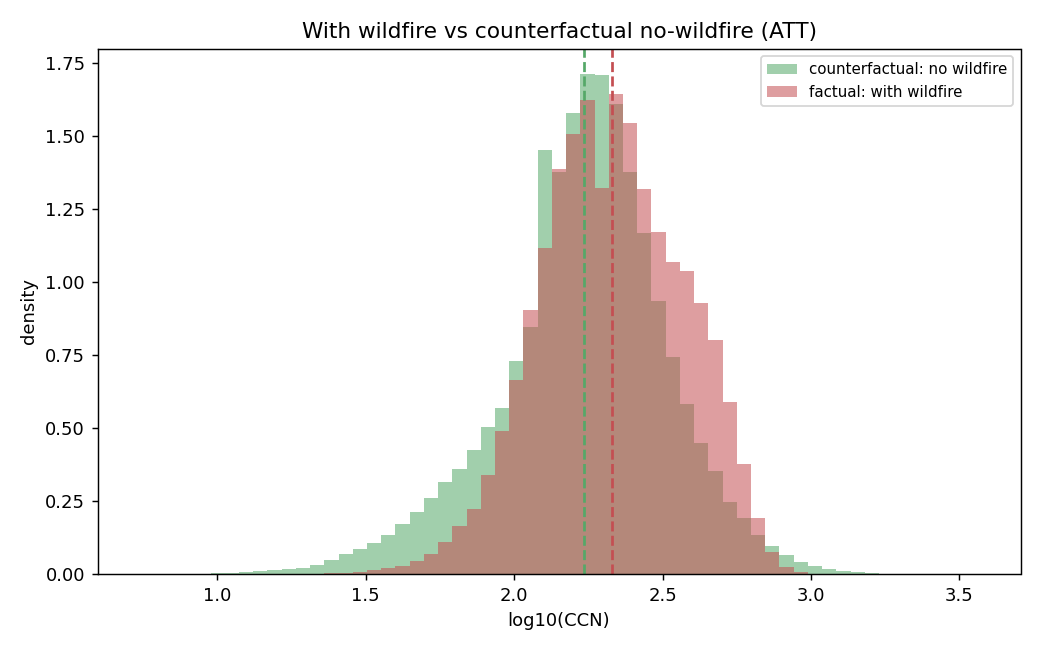
\includegraphics[width=\linewidth]{global_latent/money_plot.png}\\ \small global-latent: +24\%
\end{minipage}
\caption{CCN during wildfire periods (red) vs.\ what it would have been without
wildfire (green), for all three model types. Every one shows wildfire shifting the
distribution to higher CCN (dashed lines = averages) with a fatter high-particle
tail. Horizontal axis is a log scale. See ``How we measured it'' for exactly how
these two curves are produced.}
\label{fig:money}
\end{figure}

\section*{How we measured it}
We trained one model on wildfire periods and one on clean periods. To separate
wildfire's own effect from the weather that carried it, we compare the two models
\emph{at the same weather}. Concretely, we take the weather from the \textbf{held-out
wildfire periods} (real wildfire events the models did not train on) and run
\textbf{both} models on it:
\begin{itemize}
\item the \textbf{red} curve is the \emph{wildfire} model's predicted CCN for that
weather (``with wildfire''), and
\item the \textbf{green} curve is the \emph{clean} model's prediction for the
\emph{same} weather (``what CCN would have been without wildfire'').
\end{itemize}
Both curves use the same input (wildfire-period weather); only the model differs. The
gap between them is the wildfire effect. (We do not use the clean-period weather here
--- that would answer a different question.)

\section*{The three model types}
All three make the LSTM output a \emph{range} of possible CCN values (rather than a
single guess) by injecting Gaussian noise; they differ in where the noise enters and
how it varies across the trajectory:
\begin{itemize}
\item \textbf{Per-timestep}: a standard LSTM with a random noise vector concatenated
onto the weather inputs, redrawn \emph{fresh and independent at every timestep}.
\item \textbf{Global-latent}: the \emph{same} setup, except the noise vector is drawn
\emph{once per trajectory} and held fixed across all timesteps (one shared ``latent
code'').
\item \textbf{Recurrent}: unlike the other two, the noise is \emph{added to} the
LSTM's \emph{hidden state} (not concatenated to the inputs) at each step, so the
randomness \emph{accumulates} through the sequence.
\end{itemize}

\section*{What to keep in mind}
This is the effect during \emph{real} wildfire periods. It assumes the weather data
captures everything that differs between wildfire and clean periods, and we have not
yet attached formal error bars --- the estimate ranges from +10\% to +24\% across
model types.

\end{document}
